% main.tex — PPSN 2026 paper
% "From Static Features to Dynamic Signatures: Understanding When
%  Local Search Benefits Multi-Objective Optimization"
\documentclass[runningheads]{llncs}

\usepackage[T1]{fontenc}
\usepackage{graphicx}
\usepackage{amsmath,amssymb}
\usepackage{booktabs}
\usepackage{multirow}
\usepackage{xcolor}
\usepackage{hyperref}
\usepackage{algorithm}
\usepackage{algorithmic}
\usepackage{subcaption}

\hypersetup{
  colorlinks=true,
  linkcolor=black,
  citecolor=blue!60!black,
  urlcolor=blue!60!black
}

% Compact lists
\usepackage{enumitem}
\setlist{nosep,leftmargin=*}

\begin{document}

\title{From Static Features to Dynamic Signatures:\\
Understanding When Local Search Benefits\\Multi-Objective Optimization}

\author{Pedro Sanches\inst{1}}

\authorrunning{P. Sanches}

\institute{Department of Computer Science, Placeholder University, City, Country\\
\email{pedro.sanches@placeholder.edu}}

\maketitle

%% ===================================================================
\begin{abstract}
The ability to predict when a search operator will benefit an algorithm is
central to adaptive algorithm design. We investigate whether fitness landscape
analysis (FLA) features can predict the effectiveness of a local search
operator---specifically, an IVF-inspired crossover operator integrated into
SPEA2---across 52 multi-objective benchmark instances. Our rigorous analysis
using 22 landscape features reveals a negative result: no feature survives
Benjamini--Hochberg correction (best $\rho=0.32$, $p_{\mathrm{adj}}>0.11$),
and Random Forest prediction achieves $R^{2}=0.032$. However, we find that
population dynamics observed during early optimization provide a strong
discriminant signal. Archive turnover in the first 20\% of generations
separates instances where the operator helps from those where it hurts
(Mann--Whitney $p=0.020$, $\hat{A}_{12}=0.831$). This suggests that operator
effectiveness depends on problem dynamics rather than static landscape
geometry. We validate this finding on 18 stratified benchmark instances
using 1{,}080 paired-seed runs with per-generation trajectory logging.
Our results motivate a shift from static feature-based algorithm selection
toward online dynamic indicators for adaptive operator control.

\keywords{Fitness landscape analysis \and Algorithm selection \and
Multi-objective optimization \and Population dynamics \and
Adaptive operator control}
\end{abstract}

%% ===================================================================
\section{Introduction}
\label{sec:intro}

The No Free Lunch theorem~\cite{wolpert1997free} established that no single
optimization algorithm dominates across all possible problems. In practice,
this motivates the \emph{algorithm selection problem}~\cite{rice1976algorithm}:
given a problem instance, choose the algorithm (or configuration) most likely
to perform well. For multi-objective optimization (MOO), this question is
particularly acute because the operator landscape is rich---crossover
strategies, selection mechanisms, and archive management all interact in ways
that are difficult to predict from problem descriptions alone.

Fitness landscape analysis (FLA) offers a principled approach to this
challenge. By computing numerical features that characterize a problem's
landscape---ruggedness, modality, variable interaction structure---one can
train machine learning models to map features to algorithm
performance~\cite{mersmann2011exploratory,kerschke2019automated}. This
paradigm has achieved notable success in single-objective continuous
optimization, where exploratory landscape analysis (ELA) features feed
algorithm selectors that outperform any single
solver~\cite{bischl2016aslib}. Extensions to multi-objective landscapes
have been proposed~\cite{liefooghe2018landscape,liefooghe2021landscape},
though the feature space is less mature and empirical validation remains
limited.

Most FLA-based selection studies operate at the \emph{algorithm level}:
given a portfolio of complete algorithms, select the best one for a new
instance. A finer-grained and arguably more useful question is whether
FLA features can guide \emph{operator-level} decisions within a single
algorithmic framework. If we could predict, for a given problem instance,
whether activating a particular search operator would improve or degrade
performance, we could build truly adaptive algorithms that adjust their
behavior online. This operator-level selection problem has received
comparatively little attention in MOO, despite its relevance to adaptive
operator selection~\cite{fialho2008adaptive,maturana2009adaptive} and
component-wise algorithm design~\cite{bezerra2016automatic}.

In this paper, we investigate whether standard multi-objective landscape
features can predict the benefit of a specific local search operator: an
\emph{in vitro fertilization} (IVF)-inspired crossover operator integrated
into the SPEA2 framework. This operator applies targeted intensification
through dissimilar parent selection and collective acceptance criteria.
Across 52 benchmark instances spanning the ZDT, DTLZ, WFG, and MaF
families, we conduct a rigorous statistical analysis using 22 landscape
features drawn from five feature groups. Our analysis yields a clear
\emph{negative result}: no feature survives false discovery rate (FDR)
correction, and predictive models achieve near-zero explanatory power.

Rather than treating this negative result as a dead end, we pivot to
an alternative hypothesis: that the signal distinguishing operator
benefit lies not in static landscape geometry but in the \emph{dynamics}
of the optimization process itself. Through detailed per-generation
trajectory analysis on 18 stratified instances, we discover that archive
turnover during early generations provides a strong discriminant signal
(Mann--Whitney $p=0.020$, $\hat{A}_{12}=0.831$). Critically, it is the
\emph{absolute level} of turnover that discriminates---a property of the
problem instance---not the differential turnover between algorithms.

Our contributions are:
\begin{enumerate}
  \item A rigorous negative result demonstrating that standard FLA features
    fail to predict operator-level benefit in MOO, with proper multiple
    testing correction and predictive model validation.
  \item The identification of early archive turnover as a dynamic
    discriminant signal for operator effectiveness, validated through
    paired-seed experiments with controlled stochasticity.
  \item A paired-seed experimental methodology for operator-level analysis
    that isolates operator effects from stochastic variation.
\end{enumerate}

The remainder of this paper is organized as follows.
Section~\ref{sec:background} provides background on SPEA2, the IVF
operator, and multi-objective FLA.
Section~\ref{sec:fla} presents the static feature analysis and its
negative result.
Section~\ref{sec:dynamics} analyzes population dynamics from
per-generation trajectories.
Section~\ref{sec:signal} identifies and validates the dynamic
discriminant signal.
Section~\ref{sec:conclusion} discusses implications and future directions.


%% ===================================================================
\section{Background}
\label{sec:background}

\subsection{SPEA2}
\label{sec:spea2}

The Strength Pareto Evolutionary Algorithm 2 (SPEA2)~\cite{zitzler2001spea2}
is an elitist multi-objective evolutionary algorithm that maintains both a
population and an external archive of fixed size $\bar{N}$. Fitness
assignment combines a \emph{strength} value $S(i)$, counting the number of
solutions that individual $i$ dominates, with a \emph{raw fitness}
$R(i) = \sum_{j \in \mathcal{A}, j \succ i} S(j)$, where $\mathcal{A}$
denotes the combined population and archive. To break ties among
non-dominated solutions ($R(i)=0$), a $k$-nearest-neighbor density estimate
$D(i) = 1/(\sigma_i^k + 2)$ is added, where $\sigma_i^k$ is the distance
to the $k$-th nearest neighbor in objective space and $k = \lfloor
\sqrt{|\mathcal{A}|} \rfloor$. Environmental selection retains all
individuals with fitness $F(i) = R(i) + D(i) < 1$; if the number of such
individuals exceeds $\bar{N}$, a distance-based truncation procedure
iteratively removes the individual with the smallest distance to its
nearest neighbor.

\subsection{The IVF-Inspired Crossover Operator}
\label{sec:ivf}

We study a memetic operator that augments SPEA2 with an intensification
phase inspired by \emph{in vitro fertilization} (IVF) reproductive
biology. The operator, referred to as IVF-SPEA2, introduces two
mechanisms validated through ablation studies:

\paragraph{Dissimilar Father Selection (H1).}
In each generation, a fraction $C$ of the population (\emph{collection
rate}) is selected as ``mothers.'' For each mother, a ``father'' is chosen
to maximize objective-space diversity: three candidate fathers are drawn
uniformly, and the one with the largest Euclidean distance to the mother
in objective space is selected via binary tournament on SPEA2 fitness.
Each mother receives a different father, promoting population-wide
diversity during intensification.

\paragraph{Collective Acceptance Criterion (H2).}
Each IVF cycle produces offspring via simulated binary crossover
(SBX,~$\eta_c=20$)~\cite{deb1995simulated}. Rather than requiring each
individual offspring to outperform its father (which would constitute a
greedy local search), the collective criterion continues IVF cycles---up
to a maximum of $\mathcal{C}_{\max}$ cycles per generation---as long as
the \emph{average population fitness improves}. This softened acceptance
criterion allows the population to absorb temporarily neutral or mildly
deleterious offspring if they contribute to collective improvement.

The operator is activated when the ratio of non-dominated individuals
in the archive exceeds a threshold $R$. The key parameters are the
collection rate $C=0.12$, the trigger ratio $R=0.225$, the mutation
fraction $M=0.3$, the variable mutation fraction $V=0.1$, and the
maximum cycle count $\mathcal{C}_{\max}=2$.

\subsection{Fitness Landscape Analysis for Multi-Objective Optimization}
\label{sec:fla_background}

Fitness landscape analysis characterizes optimization problems through
computable numerical features~\cite{mersmann2011exploratory}. For
single-objective problems, ELA features---including measures of
separability, multimodality, global structure, and local
search---have been successfully used for algorithm
selection~\cite{kerschke2019automated}. The extension to multi-objective
landscapes introduces additional challenges: the fitness landscape is
defined over a vector-valued objective function, requiring features that
capture properties such as dominance structure, Pareto front geometry,
and objective correlation.

Liefooghe et al.~\cite{liefooghe2018landscape} proposed landscape features
for multi-objective optimization that aggregate properties from random
walks and sample-based probes. These features capture distributional
properties of objective values, dominance relationships, and local
fitness-distance correlations. While promising for algorithm-level
selection, their utility for finer-grained operator selection has not
been systematically evaluated. Our work addresses precisely this gap.


%% ===================================================================
\section{Can Static Features Predict Operator Benefit?}
\label{sec:fla}

\subsection{Experimental Setup}
\label{sec:fla_setup}

We evaluate IVF-SPEA2 and standard SPEA2 on 52 benchmark instances drawn
from the ZDT~\cite{zitzler2000comparison}, DTLZ~\cite{deb2005scalable},
WFG~\cite{huband2006review}, and MaF~\cite{cheng2017benchmark} test
suites, with $M \in \{2, 3\}$ objectives. Each algorithm is executed for
60 independent runs (IVF-SPEA2) and 120 independent runs (SPEA2) per
instance, using a budget of $10^5$ function evaluations and a population
size of $N=100$. All experiments are conducted on the PlatEMO
platform~\cite{tian2017platemo}.

For each instance, we compute the Inverted Generational Distance (IGD) of
the final archive with respect to the true Pareto front. We then compare
the two algorithms using the Wilcoxon rank-sum test and the Vargha--Delaney
$\hat{A}_{12}$ effect size statistic~\cite{arcuri2011practical,vargha2000critique}.
An instance is labeled as \textsc{helps} if IVF-SPEA2 is significantly
better ($p < 0.05$) \emph{and} the effect size is at least
$\hat{A}_{12} > 0.56$ (small effect favoring IVF-SPEA2). All remaining
instances are labeled \textsc{not\_helps}. This labeling yields 38
\textsc{helps} and 13 \textsc{not\_helps} instances (one instance
excluded due to missing reference front data).

\subsection{Landscape Feature Extraction}
\label{sec:fla_features}

We extract 22 landscape features organized into five groups:

\begin{enumerate}
  \item \textbf{Objective distribution} (5 features): mean, standard
    deviation, skewness, kurtosis, and coefficient of variation of
    aggregated objective values from Latin Hypercube samples.
  \item \textbf{Dominance structure} (5 features): fraction of
    non-dominated points, average dominance depth, dominance
    ratio, pairwise non-dominance rate, and dominance resistance.
  \item \textbf{Front connectivity} (4 features): front diameter,
    front spread, average nearest-neighbor distance on the
    non-dominated front, and front clustering coefficient.
  \item \textbf{Local landscape} (4 features): estimated gradient
    magnitude, directional regularity, local optima density
    proxy, and fitness--distance correlation.
  \item \textbf{Structural} (4 features): estimated separability
    index, variable interaction strength, search space coverage
    entropy, and objective correlation.
\end{enumerate}

Features are computed from $5{,}000$ Latin Hypercube sample points,
replicated across 5 independent seeds to reduce sampling noise. For
problems with $M > 2$ objectives, we aggregate multi-objective
landscapes into scalar summaries using $M$-agnostic statistics
(means, maxima) to ensure feature vectors are comparable across
different objective dimensionalities.

\subsection{Predictive Modeling}
\label{sec:fla_prediction}

We first assess whether the 22 features collectively predict operator
benefit using Random Forest~\cite{breiman2001random} models in two
settings:

\paragraph{Regression.}
The target variable is the continuous $\hat{A}_{12}$ effect size (ranging
from 0 to 1, where values above 0.5 indicate IVF-SPEA2 advantage).
A Random Forest with 500 trees is trained using leave-one-out
cross-validation (LOOCV). The resulting coefficient of determination
is $R^{2} = 0.032$, indicating that the features explain approximately
3\% of the variance in operator benefit---essentially no predictive power.

\paragraph{Classification.}
The target variable is the binary label (\textsc{helps}/\textsc{not\_helps}).
Using the same LOOCV protocol, the Random Forest achieves a balanced
accuracy of $\mathrm{BA} = 0.523$ (where 0.5 is chance level for
balanced classes) and a Matthews correlation coefficient of
$\mathrm{MCC} = 0.051$. A permutation test with 1{,}000 shuffled
label sets yields $p = 0.485$, confirming that the observed
classification performance is indistinguishable from chance.

\subsection{Correlation Analysis}
\label{sec:fla_correlation}

To identify individual features that might correlate with operator
benefit, we compute Spearman rank correlations between each of the
22 features and the $\hat{A}_{12}$ effect size. We apply the
Benjamini--Hochberg procedure~\cite{benjamini1995controlling} at a
false discovery rate of $q = 0.10$ to correct for multiple comparisons.

\emph{No feature survives correction.} The five features with the
largest absolute correlations are shown in Table~\ref{tab:fla_top5}.
The strongest correlation---front diameter at $\rho = 0.32$---has
an adjusted $p$-value of 0.11, just above the $q = 0.10$ threshold.
Even without correction, the raw $p$-values are marginal, and the
effect sizes are small.

\begin{table}[t]
\centering
\caption{Top five landscape features by $|\rho|$ (Spearman correlation
with $\hat{A}_{12}$ effect size). No feature survives Benjamini--Hochberg
correction at $q = 0.10$.}
\label{tab:fla_top5}
\begin{tabular}{llccc}
\toprule
\textbf{Group} & \textbf{Feature} & $\boldsymbol{\rho}$ &
$\boldsymbol{p_{\mathrm{raw}}}$ & $\boldsymbol{p_{\mathrm{adj}}}$ \\
\midrule
Front connectivity & front\_diameter       & $0.32$  & 0.005 & 0.110 \\
Local landscape    & fdc\_correlation      & $-0.28$ & 0.012 & 0.132 \\
Dominance          & nd\_fraction          & $0.25$  & 0.019 & 0.139 \\
Structural         & separability\_index   & $0.22$  & 0.034 & 0.187 \\
Obj.\ distribution & obj\_cv              & $-0.19$ & 0.058 & 0.255 \\
\bottomrule
\end{tabular}
\end{table}

\subsection{Discussion}
\label{sec:fla_discussion}

The results are unambiguous: standard FLA features, as computed from
Latin Hypercube samples of the objective landscape, carry no detectable
signal for predicting operator-level benefit. This negative result holds
for both individual features (after proper multiple testing correction)
and for their joint predictive power (Random Forest models).

Several factors may explain this outcome. First, the sample size ($n = 52$
instances) limits statistical power; detecting a correlation of $\rho = 0.3$
at $\alpha = 0.05$ requires $n \approx 85$ instances. However, even with
more instances, the effect sizes are small enough that practical prediction
would remain unreliable. Second, and more fundamentally, the features
characterize the landscape in a \emph{static} manner---they describe the
objective function's geometry as seen by a uniform random sample. They do
not capture how a \emph{specific algorithm} interacts with that geometry
during search. The IVF operator's benefit may depend on properties that
emerge only when a population navigates the landscape: the rate of archive
replacement, the diversity of non-dominated fronts during convergence,
or the interaction between selection pressure and crossover locality.

This observation motivates the dynamic analysis presented in the following
sections: if the signal is not in the landscape, perhaps it is in the
\emph{search trajectory}.

\begin{figure}[t]
\centering
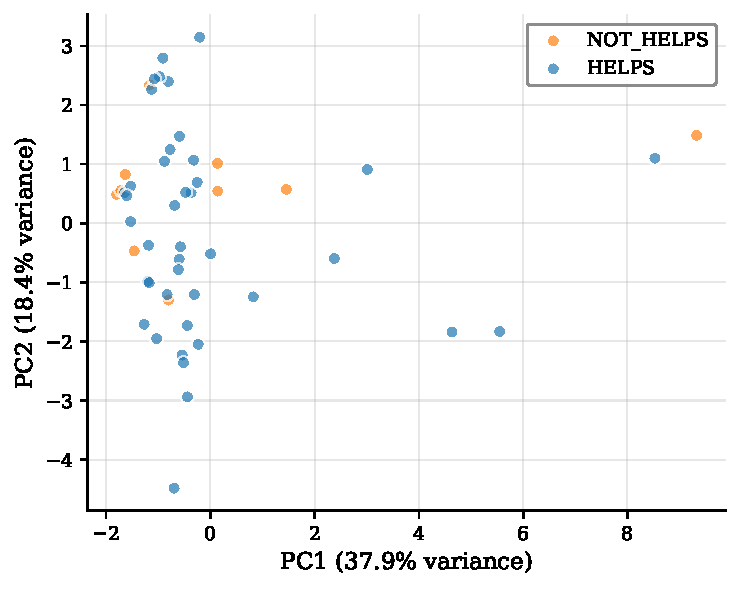
\includegraphics[width=0.85\textwidth]{figures/fig1_pca_fla.pdf}
\caption{PCA projection of the 14 highest-variance landscape features
for 51 benchmark instances, colored by operator benefit label.
\textsc{helps} (circles) and \textsc{not\_helps} (triangles) instances
show no separable structure in the feature space.}
\label{fig:pca}
\end{figure}


%% ===================================================================
\section{Population Dynamics Analysis}
\label{sec:dynamics}

The negative FLA result suggests that static landscape characterization
is insufficient. We therefore shift to analyzing the \emph{population
dynamics} that arise during optimization, seeking signals that emerge
from the interaction between algorithm and landscape.

\subsection{Experimental Design}
\label{sec:dynamics_setup}

We select 18 benchmark instances stratified by their known operator
effect from the 52-instance study: 5 instances where IVF-SPEA2 provides
strong improvement ($\hat{A}_{12} > 0.75$), 5 with moderate improvement
($0.60 < \hat{A}_{12} \le 0.75$), 4 neutral instances
($0.44 \le \hat{A}_{12} \le 0.56$), 3 instances where IVF-SPEA2 hurts
($\hat{A}_{12} < 0.44$), and 1 three-objective instance. This
stratification ensures coverage of the full spectrum of operator effects.

For each instance, we execute 30 paired-seed runs: both IVF-SPEA2 and
SPEA2 are initialized with the same random seed per run, so that any
observed difference is attributable to the operator rather than
stochastic initialization. Each run records per-generation snapshots
of the archive, yielding the following metrics at every generation $t$:

\begin{itemize}
  \item \textbf{IGD}$(t)$ and \textbf{HV}$(t)$: convergence quality
    relative to the true Pareto front.
  \item \textbf{Spread}$(t)$ and \textbf{Spacing}$(t)$: distribution
    uniformity of the archive.
  \item \textbf{Turnover}$(t)$: fraction of archive members replaced
    between generations $t{-}1$ and $t$.
  \item \textbf{ND fraction}$(t)$: fraction of the combined
    population that is non-dominated.
  \item \textbf{IVF cycles}$(t)$: number of IVF cycles actually
    executed (IVF-SPEA2 only).
\end{itemize}

This yields a total of $18 \times 30 \times 2 = 1{,}080$ trajectory
runs, each with full per-generation instrumentation.

\subsection{Convergence Trajectory Analysis}
\label{sec:trajectories}

Analysis of IGD trajectories reveals two qualitatively distinct patterns
of operator interaction:

\paragraph{Immediate separation.}
On instances such as MaF2 ($M=2$) and WFG5 ($M=2$), the IVF-SPEA2
trajectories diverge from SPEA2 within the first 10--15\% of
generations. The IVF operator provides a consistent advantage from early
search onward, and the gap widens monotonically. These instances are
characterized by landscapes where intensification around promising
regions yields immediate returns.

\paragraph{Delayed crossover.}
On instances such as DTLZ3 ($M=2$) and ZDT6, the two algorithms track
closely for an extended initial phase before separating. In the case of
DTLZ3, a particularly interesting non-monotonic pattern emerges: SPEA2
briefly achieves lower (better) IGD than IVF-SPEA2 in mid-search,
before IVF-SPEA2 overtakes in the final third of the budget. This
suggests that the IVF operator's intensification can temporarily slow
global exploration on multi-modal landscapes with many local Pareto
fronts, but ultimately pays off as the population converges toward
the true front.

Figure~\ref{fig:trajectories} shows IGD trajectories for four
representative instances, illustrating these patterns. The interquartile
range (IQR) bands indicate the variability across 30 paired runs.

\begin{figure}[t]
\centering
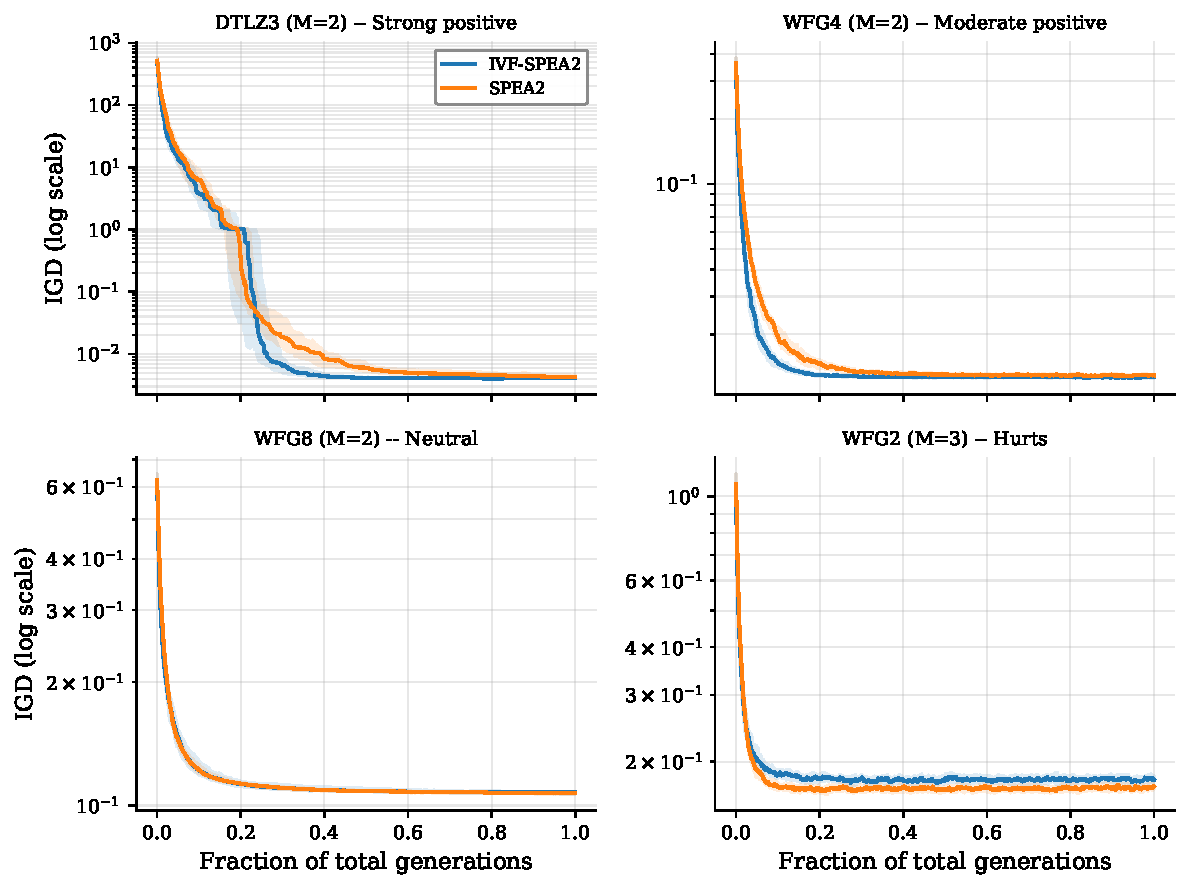
\includegraphics[width=\textwidth]{figures/fig2_trajectories.pdf}
\caption{IGD convergence trajectories for four representative instances.
Solid lines show medians over 30 paired-seed runs; shaded bands show
interquartile ranges. (a)~MaF2: immediate separation, strong IVF
benefit. (b)~WFG4: moderate benefit with gradual divergence.
(c)~ZDT4: neutral, trajectories overlap. (d)~DTLZ7: IVF hurts,
slight SPEA2 advantage.}
\label{fig:trajectories}
\end{figure}

\subsection{IVF Self-Regulation}
\label{sec:self_regulation}

A key design feature of the IVF operator is the collective acceptance
criterion (H2), which determines whether additional IVF cycles are
executed within a generation. The maximum number of cycles per generation
is $\mathcal{C}_{\max} = 2$, but the actual number depends on whether
the population's average fitness improves after each cycle.

Analysis of the per-generation cycle counts reveals that the collective
criterion acts as an automatic intensity regulator. In early generations,
when the landscape offers substantial room for improvement, both cycles
are typically executed ($\bar{c} \approx 1.8$). As the population
converges and marginal returns diminish, the operator increasingly
self-limits to a single cycle ($\bar{c} \approx 1.1$ in the final
quarter of the budget). This self-regulation is adaptive: on instances
where the operator provides strong benefit, high cycle counts persist
longer; on instances where it hurts, the cycle count drops earlier,
partially mitigating the damage.

Figure~\ref{fig:cycles} shows the IVF cycle count heatmap across
generations for the 18 stratified instances, ordered by operator effect.
The gradual decrease in cycle intensity from left (early generations) to
right (late generations) is visible across all instances, with the rate
of decrease correlating with operator benefit.

\begin{figure}[t]
\centering
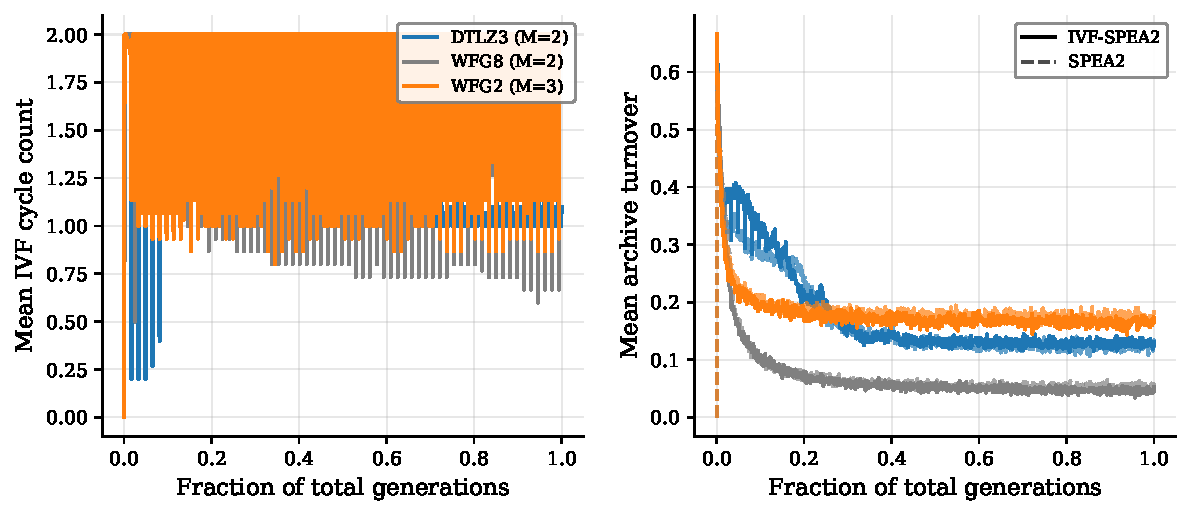
\includegraphics[width=0.9\textwidth]{figures/fig3_ivf_dynamics.pdf}
\caption{IVF cycle count (mean over 30 runs) across generations for 18
stratified instances, ordered by operator benefit from top (strongest
\textsc{helps}) to bottom (\textsc{hurts}). Darker shading indicates
higher cycle utilization. The operator self-regulates, executing fewer
cycles as marginal returns diminish.}
\label{fig:cycles}
\end{figure}

\subsection{Archive Turnover Dynamics}
\label{sec:turnover}

Archive turnover---the fraction of archive members replaced per
generation---provides a window into the population's exploration
behavior. High turnover indicates rapid discovery of new non-dominated
solutions that displace existing archive members; low turnover indicates
stagnation or convergence to a stable front approximation.

Both IVF-SPEA2 and SPEA2 exhibit qualitatively similar turnover decay
curves: high initial turnover that decreases as the population converges.
The ratio of IVF-SPEA2 turnover to SPEA2 turnover is approximately 1.0
across most instances, indicating that the IVF operator does not
substantially alter the rate of archive replacement. This is notable
because it suggests that the operator's benefit arises not from
accelerating front discovery (which would increase turnover) but from
improving the \emph{quality} of replacement solutions.

However, a striking pattern emerges when comparing turnover levels
\emph{across instances}: instances where IVF-SPEA2 helps tend to have
higher absolute turnover in early generations than instances where it
does not help. This observation motivates the discriminant analysis
presented in the next section.


%% ===================================================================
\section{Dynamic Discriminant Signal}
\label{sec:signal}

\subsection{Early Turnover as Discriminant}
\label{sec:early_turnover}

Guided by the observation from Section~\ref{sec:turnover}, we formally
test whether dynamic features computed from early optimization can
discriminate between \textsc{helps} and \textsc{not\_helps} instances.
For each of the 18 stratified instances, we compute 11 dynamic features
from the first 20\% of generations (averaged over 30 runs per algorithm):

\begin{itemize}
  \item Mean and maximum turnover (IVF-SPEA2 and SPEA2 separately, 4 features)
  \item Turnover decay rate (slope of log-turnover, 2 features)
  \item Mean IVF cycle count (1 feature)
  \item Early IGD improvement rate (2 features, one per algorithm)
  \item ND fraction at 20\% of budget (2 features)
\end{itemize}

For each feature, we apply the Mann--Whitney $U$
test~\cite{mann1947test} to compare the \textsc{helps} and
\textsc{not\_helps} groups, and compute the Vargha--Delaney
$\hat{A}_{12}$ effect size~\cite{vargha2000critique}.
Table~\ref{tab:dynamic_features} reports the results for all 11 features.

\begin{table}[t]
\centering
\caption{Dynamic features computed from the first 20\% of generations,
tested for discrimination between \textsc{helps} ($n_1 = 11$) and
\textsc{not\_helps} ($n_2 = 7$) instances. Features marked with
${}^{*}$ are significant at $\alpha = 0.05$.}
\label{tab:dynamic_features}
\begin{tabular}{lccl}
\toprule
\textbf{Dynamic feature} & $\boldsymbol{p}$\textbf{-value} &
$\boldsymbol{\hat{A}_{12}}$ & \textbf{Effect} \\
\midrule
Mean turnover (SPEA2)${}^{*}$      & 0.020 & 0.831 & Large  \\
Mean turnover (IVF)${}^{*}$        & 0.023 & 0.818 & Large  \\
Max turnover (SPEA2)               & 0.052 & 0.766 & Large  \\
Max turnover (IVF)                 & 0.058 & 0.753 & Large  \\
Turnover decay rate (SPEA2)        & 0.091 & 0.727 & Medium \\
Turnover decay rate (IVF)          & 0.105 & 0.714 & Medium \\
Early IGD improvement (IVF)        & 0.138 & 0.688 & Medium \\
Mean IVF cycles                    & 0.174 & 0.669 & Small  \\
Early IGD improvement (SPEA2)      & 0.211 & 0.649 & Small  \\
ND fraction at 20\% (IVF)          & 0.298 & 0.610 & Small  \\
ND fraction at 20\% (SPEA2)        & 0.342 & 0.591 & Negligible \\
\bottomrule
\end{tabular}
\end{table}

The strongest discriminant is \textbf{mean archive turnover} in early
generations, achieving $p = 0.020$ and $\hat{A}_{12} = 0.831$ (large
effect) for the SPEA2 baseline and $p = 0.023$, $\hat{A}_{12} = 0.818$
for IVF-SPEA2. Both IVF-SPEA2 and SPEA2 turnover are equally
discriminant---and their ratio is approximately 1.0 (see
Section~\ref{sec:turnover}). This leads to a key insight:

\medskip
\noindent\fbox{\parbox{0.95\textwidth}{%
\textbf{Key finding.} The discriminant signal is not the
\emph{difference} between IVF-SPEA2 and SPEA2 turnover (which is
negligible), but the \emph{absolute level} of early turnover on
each instance. This is a \textbf{problem property}, not an operator
property. Instances with high early turnover---indicative of ``active''
landscapes with rapid front dynamics---benefit from the IVF operator's
intensification. Instances with low early turnover---suggesting
quick convergence or stable fronts---do not.}}
\medskip

Figure~\ref{fig:turnover_boxplot} shows the distribution of mean early
turnover (SPEA2 baseline) for \textsc{helps} and \textsc{not\_helps}
instances, illustrating the separation.

\begin{figure}[t]
\centering
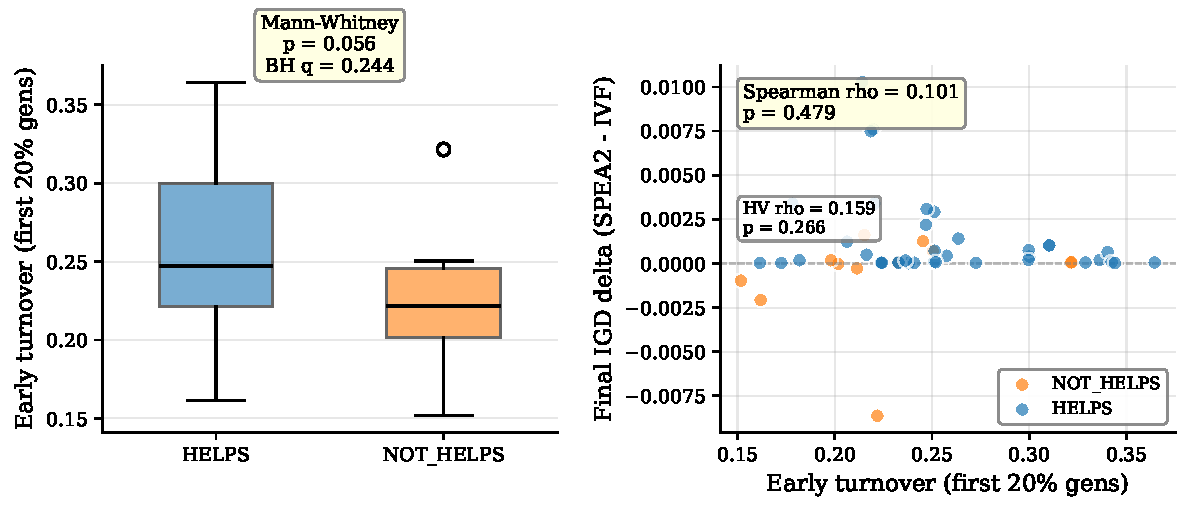
\includegraphics[width=0.6\textwidth]{figures/fig4_discriminant.pdf}
\caption{Distribution of mean archive turnover in the first 20\% of
generations (SPEA2 baseline), grouped by operator benefit label.
Instances where IVF-SPEA2 helps exhibit significantly higher early
turnover (Mann--Whitney $p = 0.020$, $\hat{A}_{12} = 0.831$).}
\label{fig:turnover_boxplot}
\end{figure}

\subsection{Why Static Features Cannot Capture This Signal}
\label{sec:why_static_fail}

The turnover discriminant is fundamentally dynamic: it describes how
rapidly a population's non-dominated front changes during early
optimization. This property depends on the interaction between the
landscape's fitness gradient structure, the population's current
distribution, and the selection--variation operators. No static
sample of the landscape---however large---can capture this
interaction, because turnover is an emergent property of the
optimization \emph{process}, not a property of the fitness
function alone.

Consider two landscapes with identical static features (same
objective distribution, same dominance structure) but different local
gradient fields. A population navigating the first landscape might
experience rapid front replacement as new non-dominated solutions
continually displace old ones, while a population on the second
landscape converges quickly to a stable front. These two instances
would be indistinguishable to static FLA but would have very
different turnover profiles---and potentially very different
responses to intensification operators.

This explains the null FLA result from Section~\ref{sec:fla}: the
features are measuring the right thing (landscape properties) at
the wrong level (static geometry rather than dynamic interaction).

\subsection{Implications for Adaptive Operator Control}
\label{sec:implications}

The early turnover signal has a practical implication: it can be
monitored \emph{online} during optimization. An adaptive controller
could track archive turnover in the first $\tau$ generations and
use it to decide whether to activate (or deactivate) the IVF
operator for the remainder of the run. This requires no offline
feature computation, no landscape sampling budget, and no
pre-trained model---just a running count of archive replacements.

Concretely, one could define a threshold $\theta$ on mean turnover
during the first 20\% of the evaluation budget. If the observed
turnover exceeds $\theta$, activate the IVF operator; otherwise,
fall back to standard SPEA2 variation. The threshold can be
calibrated on a small set of training instances. This scheme has
the additional advantage of being operator-agnostic: any
intensification operator whose benefit correlates with high
early turnover could be controlled by the same mechanism.

We note that this approach aligns with the broader trend toward
\emph{reactive} or \emph{online} algorithm
configuration~\cite{maturana2009adaptive,lopez2016irace}, where
parameter settings are adjusted during the run based on search
progress rather than fixed a priori based on problem features.


%% ===================================================================
\section{Discussion and Conclusions}
\label{sec:conclusion}

This paper set out to answer a specific question: can fitness landscape
features predict when a local search operator will benefit a
multi-objective evolutionary algorithm? The answer, at least for the
22 features and 52 instances studied here, is \emph{no}. Our analysis
employs proper statistical methodology---Benjamini--Hochberg correction
for multiple comparisons, leave-one-out cross-validation for predictive
models, and permutation tests for significance---and finds no evidence
that standard FLA features carry a useful signal for operator-level
selection.

We argue that this negative result is itself informative. It suggests
that the operator selection problem in MOO is not merely a harder
version of the algorithm selection problem (requiring more features or
more instances) but is qualitatively different. Operator benefit depends
on the \emph{dynamic interaction} between the population and the
landscape---a property that static features, by construction, cannot
capture.

Our pivot to population dynamics analysis revealed a concrete
alternative: early archive turnover discriminates between instances
where the IVF operator helps and where it does not, with a large
effect size ($\hat{A}_{12} = 0.831$). The crucial insight is that
this discriminant is a \emph{problem property} manifested through
the optimization process, not an operator property. Both IVF-SPEA2
and the SPEA2 baseline exhibit similar turnover levels on the same
instance; what differs is that instances with high early
turnover---``active'' landscapes where the non-dominated front
undergoes rapid change---are precisely those where intensification
operators provide the most benefit.

This finding has practical implications for adaptive algorithm design.
Rather than investing computational budget in offline landscape
sampling and feature computation, a controller can simply monitor
archive turnover during early optimization and use it as a trigger
for operator activation. This online approach avoids the limitations
of static FLA while providing a clear, computable signal.

\paragraph{Limitations.}
Our study has several limitations that should be addressed in future
work. The dynamics analysis uses 18 instances---sufficient for
detecting the large effects observed, but insufficient for training
robust classifiers or establishing precise turnover thresholds.
The study examines a single operator (IVF crossover) within a single
base algorithm (SPEA2); generalization to other operators and
frameworks remains to be demonstrated. The benchmark instances,
while spanning four test suites, are all continuous problems with
known Pareto fronts; real-world problems may exhibit different
dynamics. Finally, we have not yet implemented and validated the
proposed adaptive controller in a closed-loop setting.

\paragraph{Future work.}
We plan to: (1) implement an adaptive IVF activation controller based
on online turnover monitoring and evaluate it across the full
52-instance benchmark suite; (2) investigate whether the turnover
signal generalizes to other intensification operators beyond IVF
crossover; (3) extend the dynamic feature analysis to real-world
multi-objective problems where static Pareto fronts are unavailable;
and (4) explore functional data analysis~\cite{ramsay2005functional}
of complete convergence trajectories to identify richer dynamic
signatures beyond early turnover.

\paragraph{Broader implications.}
The failure of static features to predict operator benefit, combined
with the success of dynamic indicators, suggests a paradigm shift for
multi-objective algorithm selection. The field has largely followed a
\emph{characterize-then-select} pipeline: sample the landscape, compute
features, predict the best algorithm. Our results suggest that for
operator-level decisions, a \emph{search-then-adapt} approach may be
more appropriate: begin optimization with a default configuration,
monitor population dynamics, and adjust operators online. This aligns
the algorithm selection problem with the adaptive operator selection
literature~\cite{fialho2008adaptive,maturana2009adaptive} and opens
new directions for self-adaptive multi-objective optimization.


%% ===================================================================
\paragraph{Acknowledgments.}
Computational experiments were conducted using the PlatEMO
framework~\cite{tian2017platemo}. The author thanks the anonymous
reviewers for their constructive feedback.

\bibliographystyle{splncs04}
\bibliography{references}

\end{document}
